\subsection{¿Qué es Calibración de Temperatura?}

\par 
La calibración de temperatura se refiere a la calibración de cualquier dispositivo utilizado en un sistema que mide la temperatura. Generalmente hablamos del sensor de temperatura, que es típicamente un termómetro de resistencia de platino (PRT o PT-100), termistor o termopar. Las lecturas de estos termómetros se realizan mediante dispositivos de "lectura de termómetro" que miden sus salidas eléctricas y las convierten a temperatura de acuerdo con la Escala de temperatura internacional de 1990 (ITS-90).
Los termómetros suelen calibrarse colocándolos en un entorno de temperatura estable (fuente de calor) y comparando su salida con la de un "termómetro de referencia" calibrado o "termómetro estándar" \cite{temperatura-fluke}. 

\par \noindent
Por lo general las categorías generales de fuentes de calor son: fuentes de calor industriales (baño-seco, micro-baños, etc.) para uso en el campo; baños de fluidos y hornos termoeléctricos para uso en laboratorio; y células de punto fijo para calibraciones con estandares primarios.

\subsubsection{Campo, Laboratorio y Punto fijo \cite{temperatura-fluke}}

\paragraph{Calibración de Temperatura en Campo}
Tambien llamado calibración de temperatura "industrial" o "portátil", se aplica a los termómetros que se prueban fuera del entorno de laboratorio, generalmente a precisiones que van desde 5 ° C a 0,5 ° C. Pozos secos, pozos de metrología, micro-baños, objetivos de IR y otras fuentes de calor portátiles proporcionan temperaturas estables, mientras que las lecturas de termómetros portátiles y los estándares de termómetros pueden proporcionar temperaturas de referencia más allá de las disponibles directamente de la fuente de calor.

\paragraph{Calibración Secundaria o de Laboratorio}
Se refiere a la calibración de PRT o PT-100 de grado de referencia, termistores de precisión y termopares de metal noble. Baños de temperatura ultraestables y uniformes y hornos horizontales (para las altas temperaturas que necesitan los termopares) se usan junto con los termómetros de referencia SPRT y las lecturas de termómetros de alta precisión. Dichos sistemas pueden proporcionar precisiones de calibración de 0.5 ° C a 0.02 ° C.

\paragraph{Calibración Primaria o de Punto fijo} 
Utiliza celdas de punto fijo, como el punto triple de agua, que proporciona una temperatura extremadamente precisa y repetible cuando se "realizan" correctamente, normalmente en un entorno de laboratorio. Dichos sistemas se utilizan para calibrar los SPRT y los termopares de metal noble y pueden tener una precisión de 0.001 ° C.

\subsubsection{Equipos utilizados para la Calibración de Termometros}

\par 
La calibración de termometros es realizada utilizando el sistema verdadero de calibración donde el equipo a calibrar no debe estar previamente calibrado y llamamos termómetro a calibrar, al termometro (PRT, termistor o termopar) y el indicador de temperatura en conjunto.

\par \noindent
Se necesita para realizar la calibración de un termómetro: un termómetro de referencia o patrón, una fuente de temperatura, las condiciones ambientales adecuadas y el termómetro a calibrar.

\par \noindent
La norma ISO 17025:2005 indica que el termómetro de referencia debe ser más preciso, que el termómetro a calibrar; sin embargo, no especifica que superior debe ser con respecto a el termómetro a calibrar. Fluke Calibration, empresa norteamericana con acreditaciones ISO 17025 en laboratorios primarios y secundarios de temperatura, recomienda que un termómetro de referencia aceptable debe por lo menos ser 3 veces mejor, que el termómetro a calibrar.

\begin{figure}[H]
	\centering
	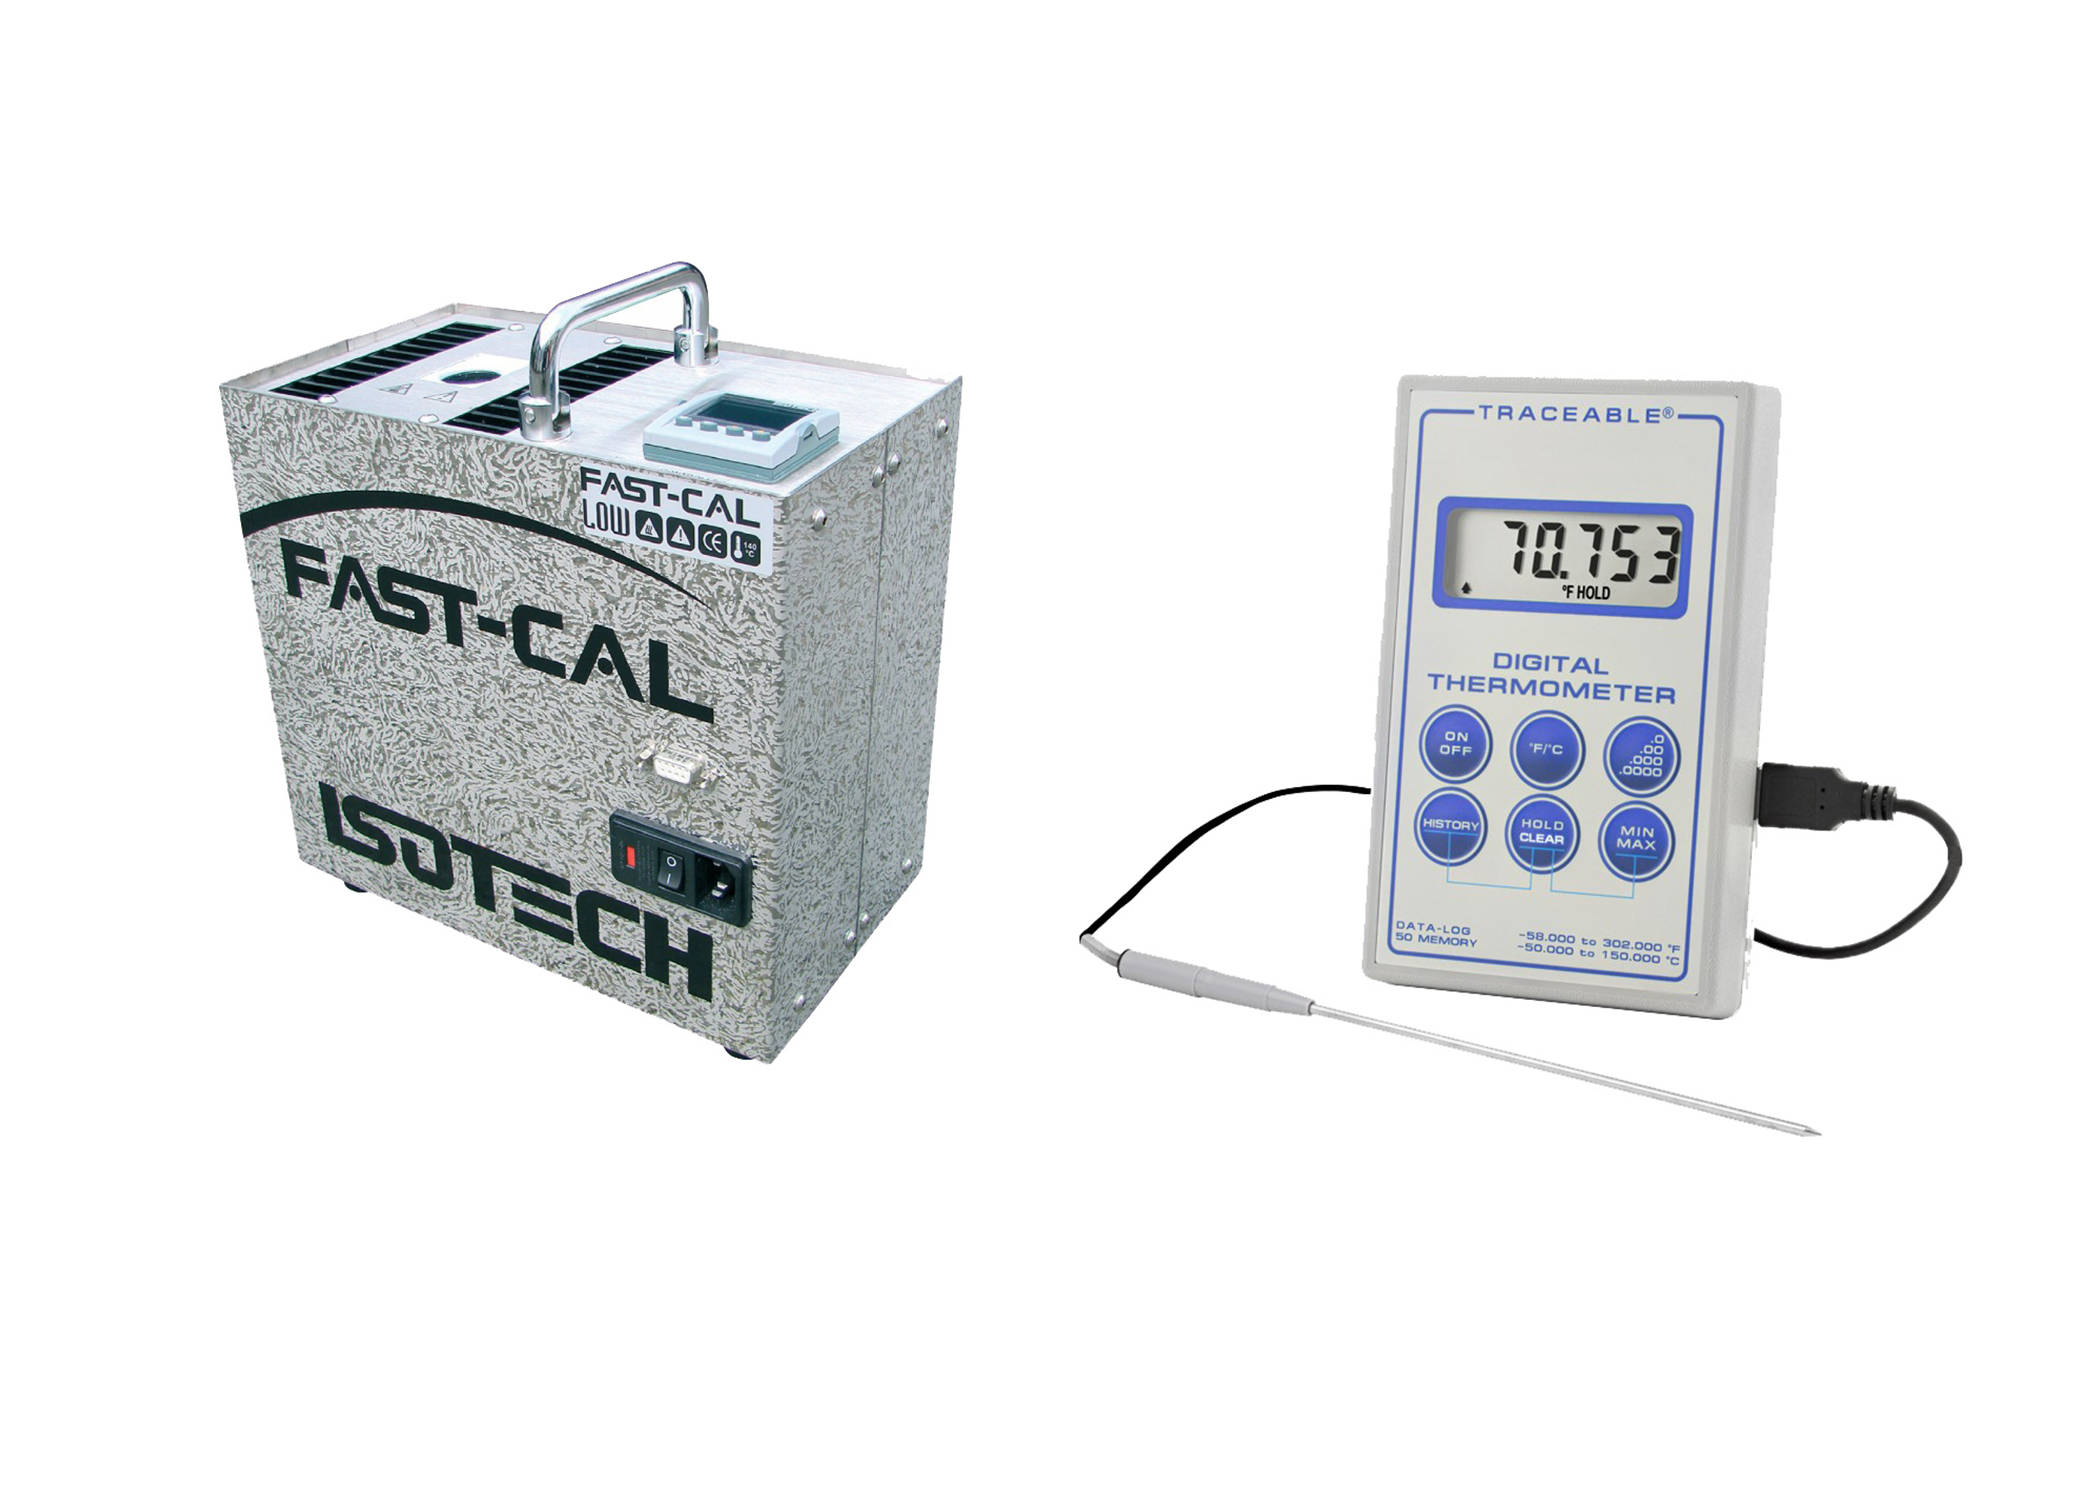
\includegraphics[width=0.6\textwidth]{caltemperatura1.png}
	\caption{Bloque de baño seco (Izquierda) y termómetro de referencia utilizado en SIGCSA (Derecha)}
\end{figure}

\par \noindent
La fuente de temperatura puede ser de 3 tipos: celdas de punto fijo, baños de fluido o calibradores de bloque seco.
Cada fuente brinda sus ventajas y desventajas. Debido a que SIGCSA realiza calibraciones en campo se utilizarán los bloques de baño seco estos nos permiten una excelente precisión en la temperatura seleccionada, es portátil y no requiere unas condiciones ambientales muy estrictas.
Adicional estos instrumentos incluyen indicadores de temperatura que son calibrados con estándares primarios.

\par \noindent
Los equipos que vayamos a utilizar dependeran del tipo de calibración de temperatura que vayamos a realizar. Los equipos utilizados en SIGCSA son excelentes para realizar calibraciones de temperatura en campo y dispositivos de grado industrial; sin embargo, si queremos realizar calibraciones de estandares secundarios o primarios, se necesitarian equipos de mayor precisión a los de grado industrial.

\begin{figure}[H]
	\centering
	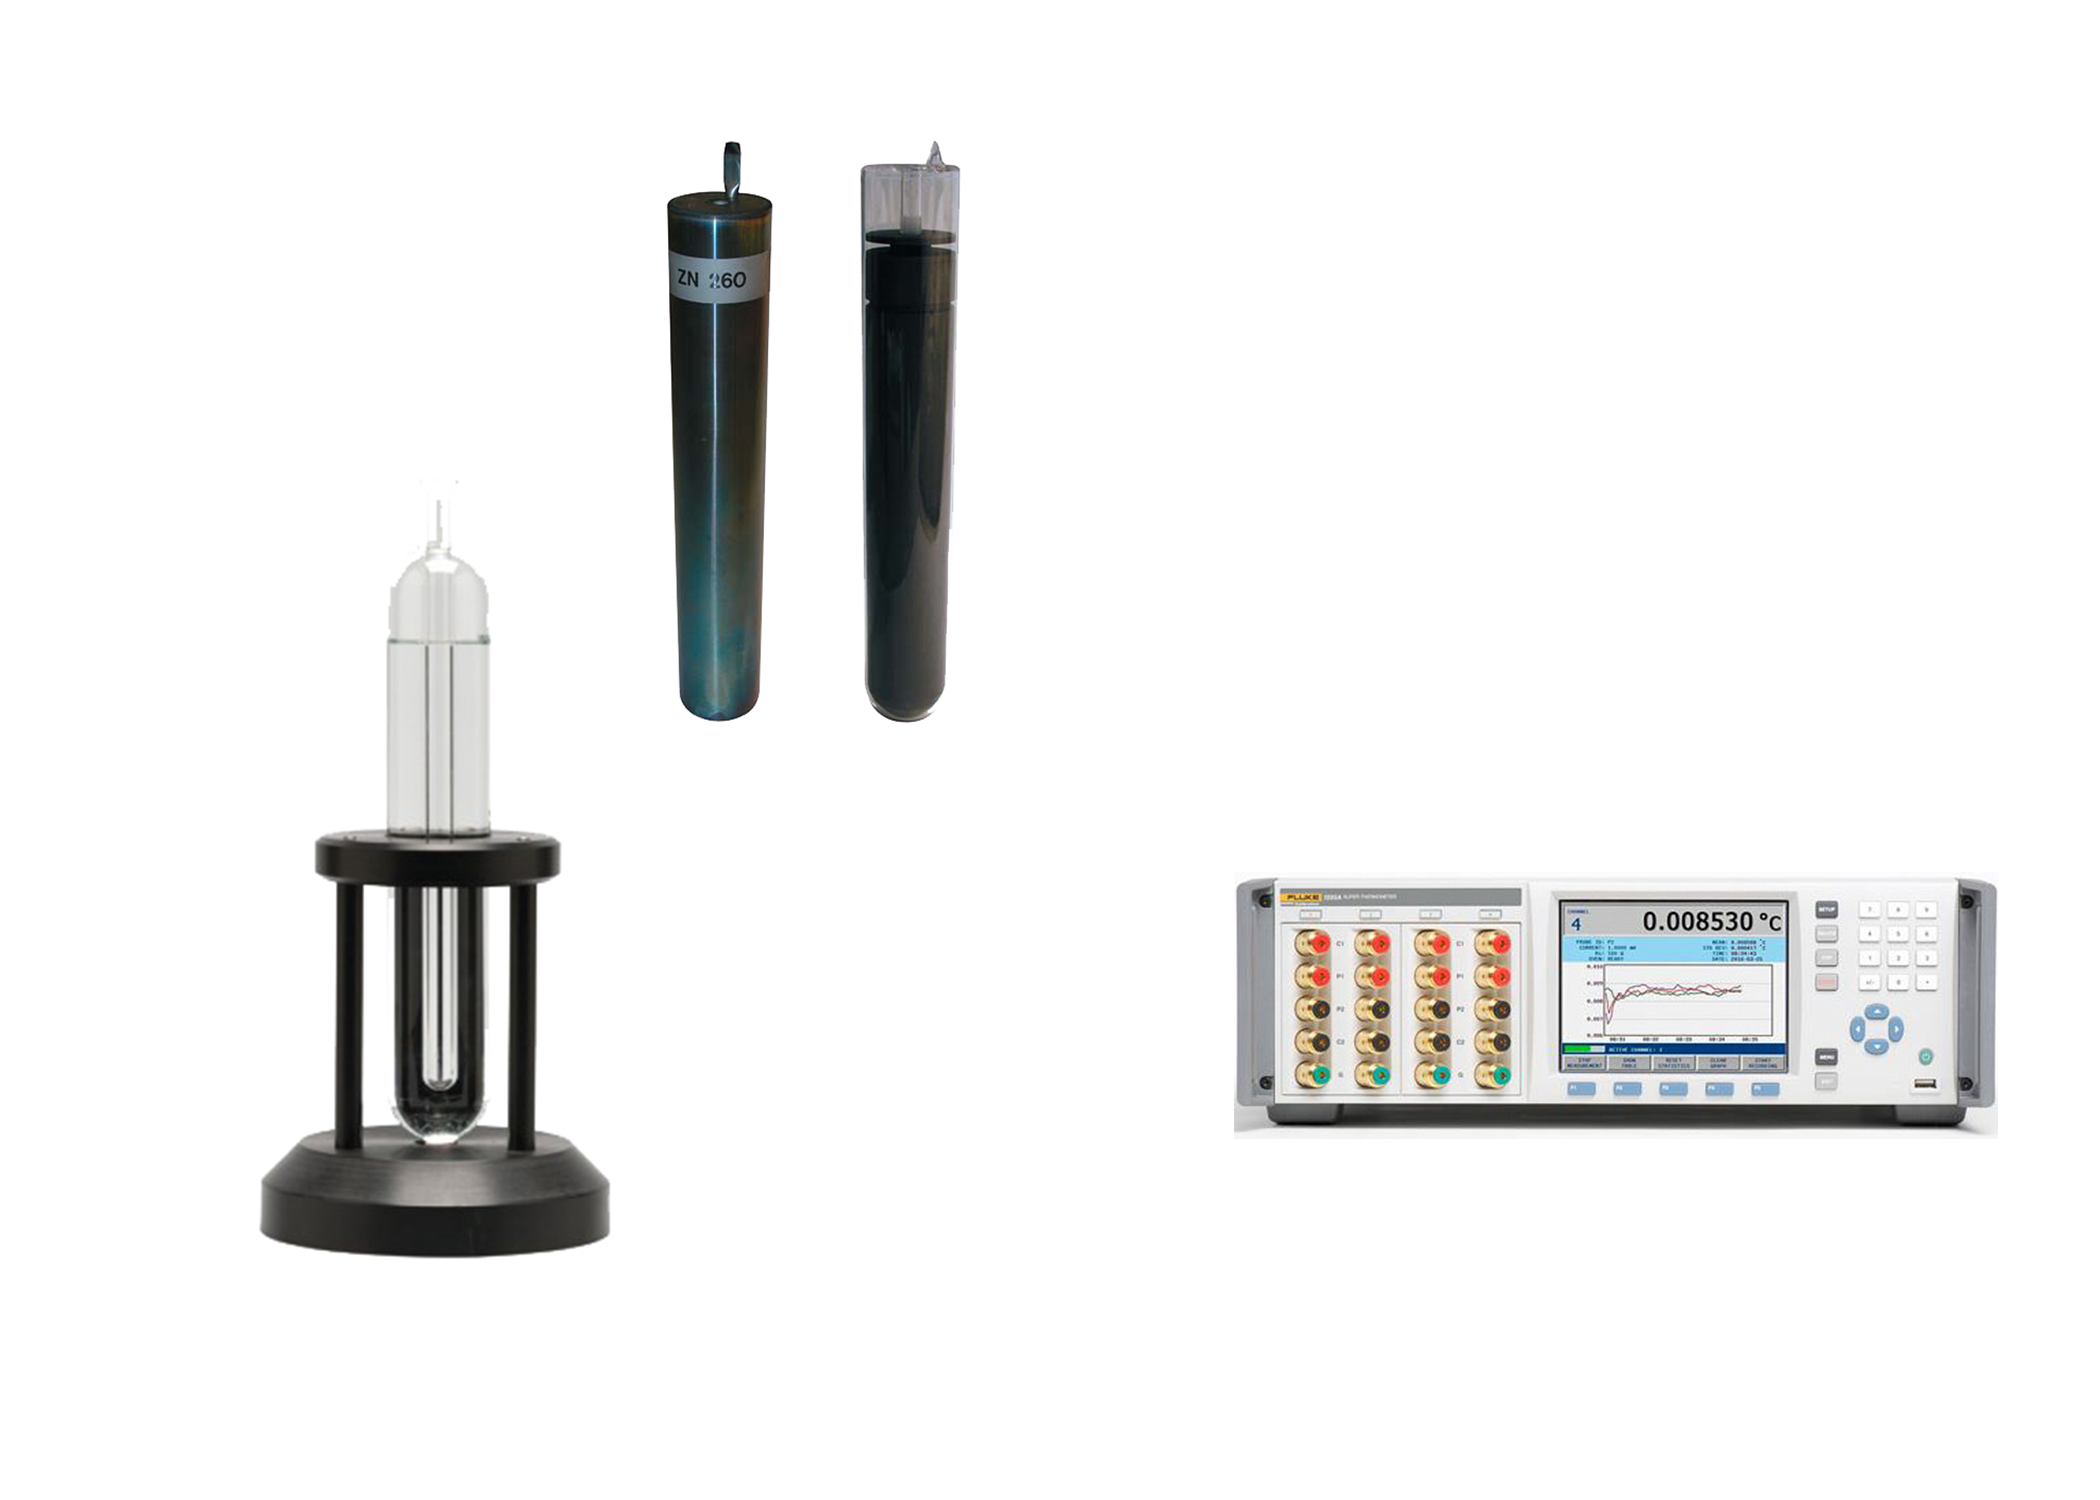
\includegraphics[width=\textwidth]{caltemperatura2.png}
	\caption{Celdas de punto fijo ITS-90 y Fluke Supertermómetro 1594A, ambos utilizados para calibraciones de estándares primarios.}
\end{figure}



